\documentclass[10pt]{article}
\usepackage[margin=1.55cm,bottom=1.3cm]{geometry}
\usepackage{booktabs,graphicx,xcolor,amsmath,textcomp}
\usepackage[T1]{fontenc}
\usepackage{lmodern}
\usepackage[stretch=15,shrink=15]{microtype}
\setlength{\parskip}{3pt}\setlength{\parindent}{0pt}
\renewcommand{\arraystretch}{1.3}
\usepackage[hidelinks]{hyperref}
\pagestyle{empty}
\newcommand{\thepar}[1]{\vspace{2.5pt}\textbf{#1}\hspace{0.7em}}
\begin{document}

\section*{1\quad Setup}

\thepar{Task and data.}A forecaster LLM predicts whether an AI model solves a benchmark task: for each pair $(t,m)$ of task $t$ and model $m$, it reports percentiles $p_{25}/p_{50}/p_{75}$ of $\Pr[\,m$ solves $t$ in one attempt$\,]$. Ground truth $y_{t,m}\in\{0,1\}$ is the recorded pass/fail from the Lyptus suite of cybersecurity benchmarks (269 usable tasks, 11-model panel, tasks grouped into 5 difficulty bins by human first-solve time). The forecaster is Claude Sonnet 4.6 at temperature 0, one call per pair. Its prompt contains example tasks with outcomes and group pass rates, all drawn from difficulty bins \emph{other than} the target's; the target's own difficulty bin is hidden.

\thepar{Splits.}Fixed once before any experiment. Search set: 84 pairs, used to select prompts during search. Held-out set: 230 pairs (21 unseen tasks $\times$ 11 models), used only for final scoring. Two whole benchmarks stay reserved for a single future out-of-distribution test.

\thepar{Metrics.}Accuracy per pair is the Brier score and, for the full percentile triple, the CRPS of a fitted Beta distribution (lower is better for both):
\begin{equation*}
\mathrm{Brier}(t,m) = \bigl(p_{50} - y_{t,m}\bigr)^2,
\qquad
\mathrm{CRPS}(F, y) = \int_0^1 \bigl(F(x) - \mathbf{1}[\,y \le x\,]\bigr)^2\,dx,
\end{equation*}
with $F$ the Beta CDF fitted to $(p_{25},p_{50},p_{75})$. A prompt's score is the mean over the 230 held-out pairs; a prompt's \emph{gain} is the paired mean difference against the seed prompt on identical pairs in the same measurement session. Output shift between two prompts is the Wasserstein-1 distance between their $p_{50}$ distributions on identical pairs. Noise floor, from re-running a fixed prompt: sd $0.0065$ for a single search-set pass, $\approx 0.002$ for a multi-pass held-out estimate.

\thepar{Baselines.}(i) The \emph{seed}: a minimal hand-written prompt holding the task statement, the evidence block, and the output format, with no forecasting guidance. Held-out Brier $0.1312$ (8 passes). (ii) The \emph{difficulty-oracle table}: no LLM, predict the leave-one-out mean pass rate of model $m$ over the other tasks in the target's difficulty bin $B(t)$,
\begin{equation*}
b(t,m) \;=\; \frac{1}{|B(t)|-1} \sum_{t' \in B(t),\, t' \neq t} y_{t',m}
\;=\; 0.1034 \text{ on the held-out set.}
\end{equation*}
The table reads the difficulty label that is hidden from the forecaster, so it is an oracle-informed reference rather than a fair competitor.

\thepar{Prompt search.}Prompts were generated with GEPA (arXiv:2507.19457), an evolutionary search in which the prompt is the only free parameter. The search keeps a pool of prompts, initialised with the seed. Each iteration samples a parent from the pool, favouring prompts that hold the best score on at least one search-set pair. An LLM rewriter (Claude Opus 4.8) reads the parent and its scored outputs on a fresh 20-pair batch and proposes a revision, which enters the pool if it outscores the parent on that batch. One run makes 40 proposals, about 4{,}000 forecaster calls. Search-set scores steer the run, but a single 84-pair pass has noise comparable to the effects, and in the replication run the prompt ranked first on the search set showed no held-out gain while the fourth-ranked prompt was the real winner. Final ranking therefore always uses $\geq 3$ full held-out passes, paired with the seed.

\section*{2\quad The prompts}

Four searches produced 82 evolved prompts; with the seed and two hand-built probes (\S3), 85 prompts total.

\begin{center}\small
\begin{tabular}{@{}p{6.3cm}cc p{5.1cm}@{}}
\toprule
source & prompts & best held-out gain & note\\
\midrule
seed (hand-written) & 1 & reference & no forecasting guidance\\[1pt]
search run 1 & 25 & $+0.027^{\star}$\; (8/8 paired passes) & ran with a scoring bug: unparsable answers scored as maximally wrong; its three winners re-verified after the fix\\[1pt]
search run 2 & 25 & $+0.016$\; (3/3) & bug fixed, otherwise identical; independent replication\\[1pt]
search variants & 32 & none beat the seed & wider acceptance test; and a rewriter told to avoid numeric content, which serves as a control in \S3\\[1pt]
single-feature probes (\S3) & 2 & $+0.020$ / $+0.006$ & seed plus exactly one feature\\
\bottomrule
\end{tabular}
\end{center}

{\footnotesize $^{\star}$the best evolved prompt; rightmost bar in the figure.}

\section*{3\quad Which prompt features matter}

Every evolved prompt was tagged for five recurring features with a fixed keyword rubric. Features arrive together in the same prompts, so the tag screen is directional evidence only; the probe experiment below is the causal test.

\begin{center}\small
\begin{tabular}{@{}lp{5.6cm}cc p{4.2cm}@{}}
\toprule
feature & what the prompt text says & n/82 & $\Delta$Brier & held-out evidence\\
\midrule
anchoring instruction & base the probability on the observed pass rates in the evidence & 82 & --- & in every evolved prompt\\
nearest-example weighting & if one example closely matches the target, weight its outcome above its group average & 31 & $-0.0043$ & in all winners; absent from the no-numbers control\\
numeric probability bands & explicit ranges per task kind: trivial lookup $0.92$--$0.99$, live exploitation $0.10$--$0.30$ & 45 & $-0.0008$ & in all winners; absent from the control; probed below\\
anti-hedging & do not default to $0.5$ when unsure & 46 & $-0.0025$ & also present in the control's null prompts\\
task-type adjustment & shift down for tasks against a live service, up for static file analysis & 69 & $-0.0029$ & near-universal, including nulls\\
\bottomrule
\end{tabular}
\end{center}

\thepar{Causal probe.}The best evolved prompt separates into numeric content (the probability bands) and a forecasting procedure (anchoring, nearest-example weighting, task-type adjustment, anti-hedging, written without any numbers). Each half was added to the seed alone and measured on the held-out set, 3 paired passes each. The bands alone recover most of the full prompt's gain ($+0.020$ of $+0.027$); the procedure alone recovers a quarter ($+0.006$). CRPS gives the same ordering (seed $0.216$, bands $0.189$, best evolved $0.178$).

\vspace{1mm}
\centerline{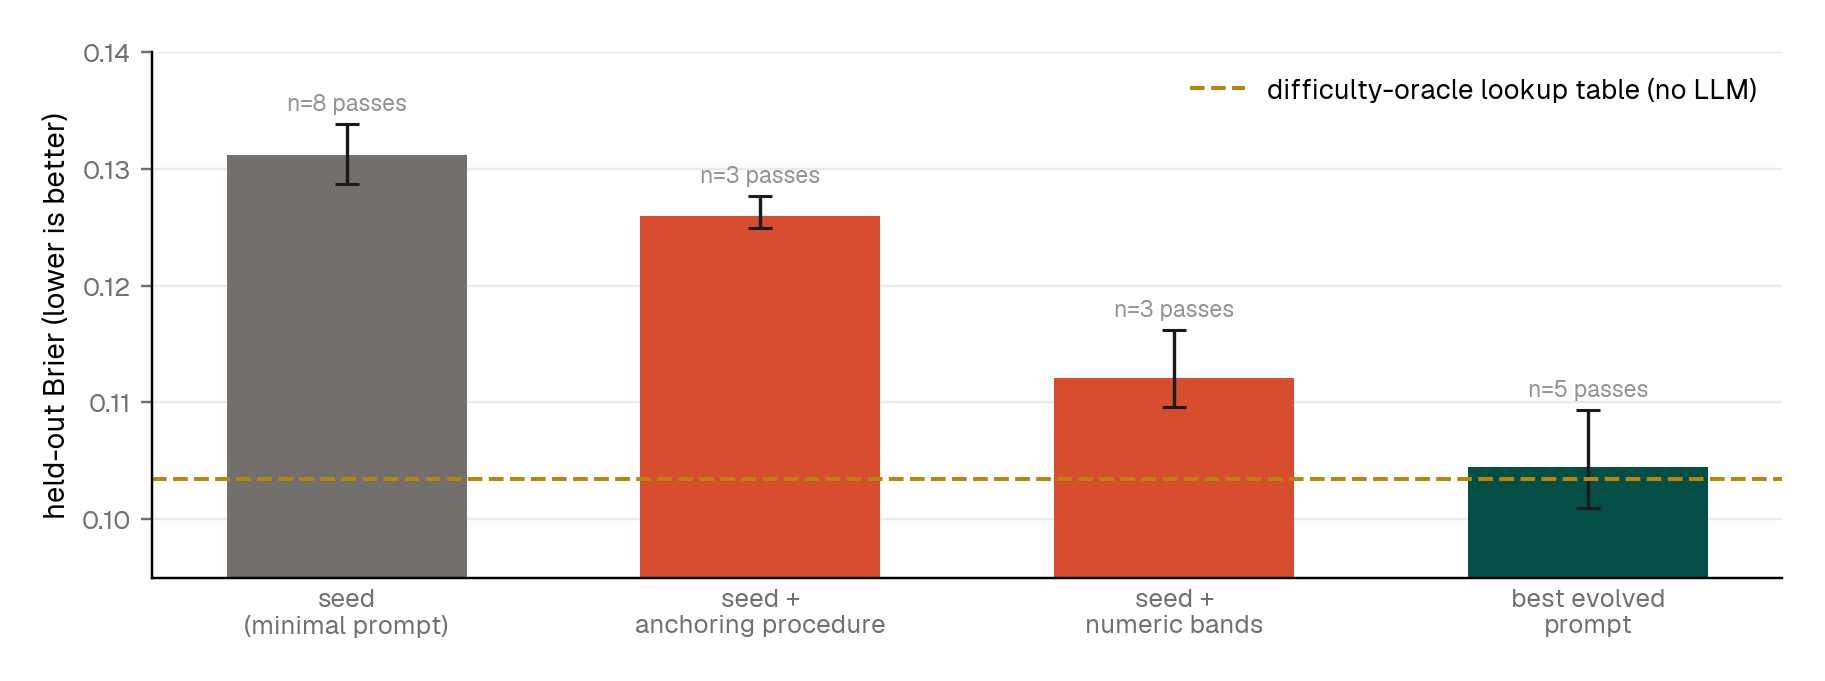
\includegraphics[width=0.62\textwidth]{fig10_feature_synthesis.png}}
\vspace{0.5mm}

\section*{4\quad Conclusions}

\thepar{1. Numeric anchors in the prompt do the work.}Adding the winner's numbers to the seed recovers about three quarters of its gain; adding the same procedure with the numbers removed recovers a quarter. This agrees with the spring elicitation studies, where model outputs followed whatever number the prompt supplied and removing anchors mainly increased variance. For this task, prompt design reduces to choosing which numbers the model sees; instructions that tell the model how to derive its own numbers are a weak substitute.

\thepar{2. A lookup table bounds what optimization buys.}The search improved the forecaster in two independent runs, in both cases by improving discrimination rather than calibration. The best evolved prompt matches the difficulty-oracle table and does not beat it, and the strongest base model tested in the spring reached the same level from a hand-written prompt. Within the training distribution the table is the practical ceiling, and optimization recovered about one model generation of accuracy.

\thepar{3. The open question is transfer.}A lookup table cannot extrapolate to unseen benchmarks. Whether the evolved prompt can is the remaining question, and the reserved benchmarks exist for that single test.

\vspace{1.5mm}
{\scriptsize\raggedright\emph{Reproducibility.} Scripts \texttt{feature\_report\_data.py}, \texttt{val\_noise\_study.py}, \texttt{parse\_failure\_audit.py} (gepa repo); raw runs on \texttt{results/*} branches; curated data, prompt texts, this document: \texttt{experiments/III\_gepa\_optimization/summary/}; earlier stages: \texttt{prompt\_sensitivity/}, experiments I/II, final report \S3. 2026-08-30.\par}

\end{document}
